%# -*- coding: utf-8 -*-
%!TEX encoding = UTF-8 Unicode
%!TEX TS-program = xelatex
% vim:ts=4:sw=4
%
% 以上设定默认使用 XeLaTex 编译,并指定 Unicode 编码,供 TeXShop 自动识别

% Author: Yunhui Fu <yhfudev@gmail.com>
% License: Creative Commons (CC BY 4.0)

\section{Using the MNIST Dataset} \label{chp:usemnistdata}

\subsection{Introduction}
The MNIST dataset is a dataset of handwritten digits, comprising 60 000 training examples and 10 000 test examples. The dataset can be downloaded from \url{http://yann.lecun.com/exdb/mnist/}.

\subsection{Usage}

The image and label data is stored in a binary format described on the website. For your convenience, we have provided two MATLAB helper functions for extracting the data. These functions are available at \url{http://ufldl.stanford.edu/wiki/resources/mnistHelper.zip}.

As an example of how to use these functions, you can check the images and labels using the following code:
\begin{lstlisting}[language=matlab]
% Change the filenames if you've saved the files under different names
% On some platforms, the files might be saved as
% train-images.idx3-ubyte / train-labels.idx1-ubyte
images = loadMNISTImages('train-images-idx3-ubyte');
labels = loadMNISTLabels('train-labels-idx1-ubyte');

% We are using display_network from the autoencoder code
display_network(images(:,1:100)); % Show the first 100 images
disp(labels(1:10));
\end{lstlisting}






\section{\cnt{Miscellaneous Topics}{}{}}

\subsection{\cnt{Data Preprocessing}{数据预处理}{}}

\subsubsection{\cnt{Overview}{概要}{}}

\cnt{Data preprocessing plays a very important in many deep learning algorithms. In practice, many methods work best after the data has been normalized and whitened. However, the exact parameters for data preprocessing are usually not immediately apparent unless one has much experience working with the algorithms. In this page, we hope to demystify some of the preprocessing methods and also provide tips (and a ``standard pipeline") for preprocessing data.}
    {数据预处理在众多深度学习算法中都起着重要作用,实际情况中,将数据做归一化和白化处理后,很多算法能够发挥最佳效果。然而除非对这些算法有丰富的使用经验,否则预处理的精确参数并非显而易见。在本页中,我们希望能够揭开预处理方法的神秘面纱,同时为预处理数据提供技巧(和标准流程)。}
    {}

%\notes{
\cnt{Tip: When approaching a dataset, the first thing to do is to look at the data itself and observe its properties. While the techniques here apply generally, you might want to opt to do certain things differently given your dataset. For example, one standard preprocessing trick is to subtract the mean of each data point from itself (also known as remove DC, local mean subtraction, subtractive normalization). While this makes sense for data such as natural images, it is less obvious for data where stationarity does not hold.}
    {提示:当我们开始处理数据时,首先要做的事是观察数据并获知其特性。本部分将介绍一些通用的技术,在实际中应该针对具体数据选择合适的预处理技术。例如一种标准的预处理方法是对每一个数据点都减去它的均值(也被称为移除直流分量,局部均值消减,消减归一化),这一方法对诸如自然图像这类数据是有效的,但对非平稳的数据则不然。}
    {}
%} notes

\subsubsection{\cnt{Data Normalization}{数据归一化}{}}

\cnt{A standard first step to data preprocessing is data normalization. While there are a few possible approaches, this step is usually clear depending on the data. The common methods for feature normalization are:}
    {数据预处理中,标准的第一步是数据归一化。虽然这里有一系列可行的方法,但是这一步通常是根据数据的具体情况而明确选择的。特征归一化常用的方法包含如下几种:}
    {}

\begin{itemize}
  \item \cnt{Simple Rescaling}{简单缩放}{}
  \item \cnt{Per-example mean subtraction (a.k.a. remove DC)}{逐样本均值消减(也称为移除直流分量)}{}
  \item \cnt{Feature Standardization (zero-mean and unit variance for each feature across the dataset)}{特征标准化(使数据集中所有特征都具有零均值和单位方差)}{}
\end{itemize}

\textbf{\cnt{Simple Rescaling}{简单缩放}{}}

\cnt{In simple rescaling, our goal is to rescale the data along each data dimension (possibly independently) so that the final data vectors lie in the range $[0,1]$ or $[ - 1,1]$ (depending on your dataset). This is useful for later processing as many \emph{default} parameters (e.g., \texttt{epsilon} in PCA-whitening) treat the data as if it has been scaled to a reasonable range.}
    {在简单缩放中,我们的目的是通过对数据的每一个维度的值进行重新调节(这些维度可能是相互独立的),使得最终的数据向量落在 [0,1]或[ - 1,1] 的区间内(根据数据情况而定)。这对后续的处理十分重要,因为很多\emph{默认}参数(如 PCA-白化中的 \texttt{epsilon})都假定数据已被缩放到合理区间。}
    {}

\cnt{\textbf{Example}: When processing natural images, we often obtain pixel values in the range [0,255]. It is a common operation to rescale these values to [0,1] by dividing the data by 255.}
    {例子:在处理自然图像时,我们获得的像素值在 [0,255] 区间中,常用的处理是将这些像素值除以 255,使它们缩放到 [0,1] 中.}
    {}


\textbf{\cnt{Per-example mean subtraction}{逐样本均值消减}{}}

\cnt{If your data is \emph{stationary} (i.e., the statistics for each data dimension follow the same distribution), then you might want to consider subtracting the mean-value for each example (computed per-example).}
    {如果你的数据是\emph{平稳的}(即数据每一个维度的统计都服从相同分布),那么你可以考虑在每个样本上减去数据的统计平均值(逐样本计算)。}
    {}

\cnt{\textbf{Example}: In images, this normalization has the property of removing the average brightness (intensity) of the data point. In many cases, we are not interested in the illumination conditions of the image, but more so in the content; removing the average pixel value per data point makes sense here. Note: While this method is generally used for images, one might want to take more care when applying this to color images. In particular, the stationarity property does not generally apply across pixels in different color channels.}
    {例子:对于图像,这种归一化可以移除图像的平均亮度值 (intensity)。很多情况下我们对图像的照度并不感兴趣,而更多地关注其内容,这时对每个数据点移除像素的均值是有意义的。注意:虽然该方法广泛地应用于图像,但在处理彩色图像时需要格外小心,具体来说,是因为不同色彩通道中的像素并不都存在平稳特性。}
    {}


\textbf{\cnt{Feature Standardization}{特征标准化}{}}

\cnt{Feature standardization refers to (independently) setting each dimension of the data to have zero-mean and unit-variance. This is the most common method for normalization and is generally used widely (e.g., when working with SVMs, feature standardization is often recommended as a preprocessing step). In practice, one achieves this by first computing the mean of each dimension (across the dataset) and subtracts this from each dimension. Next, each dimension is divided by its standard deviation.}
    {特征标准化指的是(独立地)使得数据的每一个维度具有零均值和单位方差。这是归一化中最常见的方法并被广泛地使用(例如,在使用支持向量机(SVM)时,特征标准化常被建议用作预处理的一部分)。在实际应用中,特征标准化的具体做法是:首先计算每一个维度上数据的均值(使用全体数据计算),之后在每一个维度上都减去该均值。下一步便是在数据的每一维度上除以该维度上数据的标准差。}
    {}

\cnt{\textbf{Example}: When working with audio data, it is common to use \href{http://en.wikipedia.org/wiki/Mel-frequency_cepstrum}{MFCCs} as the data representation. However, the first component (representing the DC) of the MFCC features often overshadow the other components. Thus, one method to restore balance to the components is to standardize the values in each component independently.}
    {例子:处理音频数据时,常用 Mel 倒频系数 MFCCs 来表征数据。然而MFCC特征的第一个分量(表示直流分量)数值太大,常常会掩盖其他分量。这种情况下,为了平衡各个分量的影响,通常对特征的每个分量独立地使用标准化处理。}
    {}



\subsubsection{\cnt{PCA/ZCA Whitening}{PCA/ZCA白化}{}}

\cnt{After doing the simple normalizations, whitening is often the next preprocessing step employed that helps make our algorithms work better. In practice, many deep learning algorithms rely on whitening to learn good features.}
    {在做完简单的归一化后,白化通常会被用来作为接下来的预处理步骤,它会使我们的算法工作得更好。实际上许多深度学习算法都依赖于白化来获得好的特征。}
    {}

\cnt{In performing PCA/ZCA whitening, it is pertinent to first zero-mean the features (across the dataset) to ensure that $\frac{1}{m} \sum_i x^{(i)} = 0$. Specifically, this should be done before computing the covariance matrix. (The only exception is when per-example mean subtraction is performed and the data is stationary across dimensions/pixels.)}
    {在进行 PCA/ZCA 白化时,首先使特征零均值化是很有必要的,这保证了 $\frac{1}{m} \sum_i x^{(i)} = 0$。特别地,这一步需要在计算协方差矩阵前完成。(唯一例外的情况是已经进行了逐样本均值消减,并且数据在各维度上或像素上是平稳的。)}
    {}

\cnt{Next, one needs to select the value of \texttt{epsilon} to use when performing PCA/ZCA whitening(\ref{chp:whitening}) (recall that this was the regularization term that has an effect of \emph{low-pass filtering} the data). It turns out that selecting this value can also play an important role for feature learning, we discuss two cases for selecting \texttt{epsilon}:}
    {接下来在 PCA/ZCA 白化(\ref{chp:whitening})中我们需要选择合适的 \texttt{epsilon}(回忆一下,这是规则化项,对数据有低通滤波作用)。 选取合适的 \texttt{epsilon} 值对特征学习起着很大作用,下面讨论在两种不同场合下如何选取 \texttt{epsilon}:}
    {}

\textbf{\cnt{Reconstruction Based Models}{基于重构的模型}{}}

\cnt{In models based on reconstruction (including Autoencoders, Sparse Coding, RBMs, k-Means), it is often preferable to set \texttt{epsilon} to a value such that low-pass filtering is achieved. One way to check this is to set a value for \texttt{epsilon}, run ZCA whitening, and thereafter visualize the data before and after whitening. If the value of \texttt{epsilon} is set too low, the data will look very noisy; conversely, if \texttt{epsilon} is set too high, you will see a ``blurred" version of the original data. A good way to get a feel for the magnitude of \texttt{epsilon} to try is to plot the eigenvalues on a graph. As visible in the example graph below, you may get a ``long tail" corresponding to the high frequency noise components. You will want to choose \texttt{epsilon} such that most of the ``long tail" is filtered out, i.e. choose \texttt{epsilon} such that it is greater than most of the small eigenvalues corresponding to the noise.}
    {在基于重构的模型中(包括自编码器,稀疏编码,受限 Boltzman 机(RBM),k-均值(K-Means)),经常倾向于选取合适的 \texttt{epsilon} 以使得白化达到低通滤波的效果。(译注:通常认为数据中的高频分量是噪声,低通滤波的作用就是尽可能抑制这些噪声,同时保留有用的信息。在 PCA 等方法中,假设数据的信息主要分布在方差较高的方向,方差较低的方向是噪声(即高频分量),因此后文中 \texttt{epsilon} 的选择与特征值有关)。一种检验 \texttt{epsilon} 是否合适的方法是用该值对数据进行 ZCA 白化,然后对白化前后的数据进行可视化。如果 \texttt{epsilon} 值过低,白化后的数据会显得噪声很大;相反,如果 \texttt{epsilon} 值过高,白化后的数据与原始数据相比就过于模糊。一种直观上得到 \texttt{epsilon} 大小的方法是以图形方式画出数据的特征值,如下图的例子所示,你可以看到一条``长尾",它对应于数据中的高频噪声部分。你需要选取合适的 \texttt{epsilon},使其能够在很大程度上过滤掉这条``长尾",也就是说,选取的 \texttt{epsilon} 应大于大多数较小的、反映数据中噪声的特征值。}
    {}

\begin{figure}[ht] \centering
  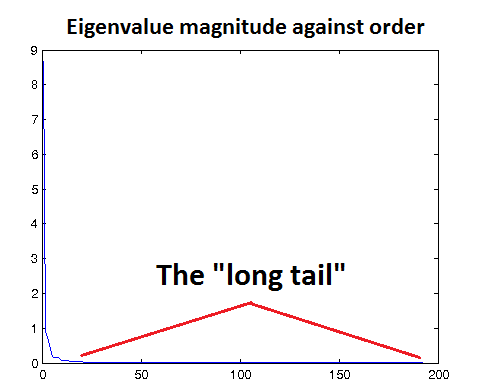
\includegraphics[width=0.5\textwidth]{figures/ZCA_Eigenvalues_Plot.png}
  %\caption{}\label{fig:step1}
\end{figure}

\cnt{In reconstruction based models, the loss function includes a term that penalizes reconstructions that are far from the original inputs. Then, if \texttt{epsilon} is set too low, the data will contain a lot of noise which the model will need to reconstruct well. As a result, it is very important for reconstruction based models to have data that has been low-pass filtered.}
    {在基于重构的模型中,损失函数有一项是用于惩罚那些与原始输入数据差异较大的重构结果(译注:以自动编码机为例,要求输入数据经过编码和解码之后还能尽可能的还原输入数据)。如果 \texttt{epsilon} 太小,白化后的数据中就会包含很多噪声,而模型要拟合这些噪声,以达到很好的重构结果。因此,对于基于重构的模型来说,对原始数据进行低通滤波就显得非常重要。}
    {}

\cnt{Tip: If your data has been scaled reasonably (e.g., to [0,1]), start with \texttt{epsilon = 0.01} or \texttt{epsilon = 0.1}.}
    {提示:如果数据已被缩放到合理范围(如[0,1]),可以从 \texttt{epsilon = 0.01} 或 \texttt{epsilon = 0.1} 开始调节 \texttt{epsilon}。}
    {}

\textbf{\cnt{ICA-based Models (with orthogonalization)}{基于正交化ICA的模型}{}}

\cnt{For ICA-based models with orthogonalization, it is very important for the data to be as close to white (identity covariance) as possible. This is a side-effect of using orthogonalization to decorrelate the features learned (more details in ICA \ref{chp:indepcomponanalysis}). Hence, in this case, you will want to use an \texttt{epsilon} that is as small as possible (e.g., \texttt{epsilon = 1e - 6}).}
    {基于正交化ICA的模型来说,保证输入数据尽可能地白化(即协方差矩阵为单位矩阵)非常重要。这是因为:这类模型需要对学习到的特征做正交化,以解除不同维度之间的相关性(详细内容请参考 ICA \ref{chp:indepcomponanalysis} 一节)。因此在这种情况下,\texttt{epsilon} 要足够小(比如 \texttt{epsilon = 1e - 6})。}
    {}

\cnt{Tip: In PCA whitening, one also has the option of performing dimension reduction while whitening the data. This is usually an excellent idea since it can greatly speed up the algorithms (less computation and less parameters). A simple rule of thumb to choose how many principle components to retain is to keep enough components to have 99\% of the variance retained (more details at PCA \ref{chp:pcaselectnum})}
    {提示:我们也可以在PCA白化过程中同时降低数据的维度。这是一个很好的主意,因为这样可以大大提升算法的速度(减少了运算量和参数数目)。确定要保留的主成分数目有一个经验法则:即所保留的成分的总方差达到总样本方差的 99\% 以上。(详细内容请参考 PCA \ref{chp:pcaselectnum} )}
    {}

\cnt{Note: When working in a classification framework, one should compute the PCA/ZCA whitening matrices based only on the training set. The following parameters used be saved for use with the test set: (a) average vector that was used to zero-mean the data, (b) whitening matrices. The test set should undergo the same preprocessing steps using these saved values.}
    {注意: 在使用分类框架时,我们应该只基于练集上的数据计算PCA/ZCA白化矩阵。需要保存以下两个参数留待测试集合使用:(a)用于零均值化数据的平均值向量;(b)白化矩阵。测试集需要采用这两组保存的参数来进行相同的预处理。}
    {}

\subsubsection{\cnt{Large Images}{大图像}{}}

\cnt{For large images, PCA/ZCA based whitening methods are impractical as the covariance matrix is too large. For these cases, we defer to 1/f-whitening methods. (more details to come)}
    {对于大图像,采用基于 PCA/ZCA 的白化方法是不切实际的,因为协方差矩阵太大。在这些情况下我们退而使用 1/f 白化方法(更多内容后续再讲)。}
    {}



\subsubsection{\cnt{Standard Pipelines}{标准流程}{}}

\cnt{In this section, we describe several ``standard pipelines" that have worked well for some datasets:}
    {在这一部分中,我们将介绍几种在一些数据集上有良好表现的预处理标准流程.}
    {}


\textbf{\cnt{Natural Grey-scale Images}{自然灰度图像}{}}

\cnt{Since grey-scale images have the stationarity property, we usually first remove the mean-component from each data example separately (remove DC). After this step, PCA/ZCA whitening is often employed with a value of \texttt{epsilon} set large enough to low-pass filter the data.}
    {灰度图像具有平稳特性,我们通常在第一步对每个数据样本分别做均值消减(即减去直流分量),然后采用 PCA/ZCA 白化处理,其中的 \texttt{epsilon} 要足够大以达到低通滤波的效果。}
    {}

\textbf{\cnt{Color Images}{彩色图像}{}}

\cnt{For color images, the stationarity property does not hold across color channels. Hence, we usually start by rescaling the data (making sure it is in [0,1]) ad then applying PCA/ZCA with a sufficiently large \texttt{epsilon}. Note that it is important to perform feature mean-normalization before computing the PCA transformation.}
    {对于彩色图像,色彩通道间并不存在平稳特性。因此我们通常首先对数据进行特征缩放(使像素值位于 [0,1] 区间),然后使用足够大的 \texttt{epsilon} 来做 PCA/ZCA。注意在进行 PCA 变换前需要对特征进行分量均值归零化。}
    {}

\textbf{\cnt{Audio (MFCC/Spectrograms)}{音频 (MFCC/频谱图)}{}}

\cnt{For audio data (MFCC and Spectrograms), each dimension usually have different scales (variances); the first component of MFCCs, for example, is the DC component and usually has a larger magnitude than the other components. This is especially so when one includes the temporal derivatives (a common practice in audio processing). As a result, the preprocessing usually starts with simple data standardization (zero-mean, unit-variance per data dimension), followed by PCA/ZCA whitening (with an appropriate \texttt{epsilon}).}
    {对于音频数据 (MFCC 和频谱图),每一维度的取值范围(方差)不同。例如 MFCC 的第一分量是直流分量,通常其幅度远大于其他分量,尤其当特征中包含时域导数 (temporal derivatives) 时(这是音频处理中的常用方法)更是如此。因此,对这类数据的预处理通常从简单的数据标准化开始(即使得数据的每一维度均值为零、方差为 1),然后进行 PCA/ZCA 白化(使用合适的 \texttt{epsilon})。}
    {}

\textbf{\cnt{MNIST Handwritten Digits}{MNIST 手写数字}{}}

\cnt{The MNIST dataset has pixel values in the range [0,255]. We thus start with simple rescaling to shift the data into the range [0,1]. In practice, removing the mean-value per example can also help feature learning. Note: While one could also elect to use PCA/ZCA whitening on MNIST if desired, this is not often done in practice.}
    {MNIST 数据集的像素值在 [0,255] 区间中。我们首先将其缩放到 [0,1] 区间。实际上,进行逐样本均值消去也有助于特征学习。注:也可选择以对 MNIST 进行 PCA/ZCA 白化,但这在实践中不常用。}
    {}


\subsection{\cnt{Deriving gradients using the backpropagation idea}{用反向传导思想求导}{}} \label{chp:derivegradbackpropidea}


\subsubsection{\cnt{Introduction}{简介}{}}

\cnt{In the section on the backpropagation algorithm (\ref{chp:bkpropgationalg}), you were briefly introduced to backpropagation as a means of deriving gradients for learning in the sparse autoencoder. It turns out that together with matrix calculus, this provides a powerful method and intuition for deriving gradients for more complex matrix functions (functions from matrices to the reals, or symbolically, from $\mathbb{R}^{r \times c} \rightarrow \mathbb{R}$).}
    {在 反向传导算法(\ref{chp:bkpropgationalg}) 一节中,我们介绍了在稀疏自编码器中用反向传导算法来求梯度的方法。事实证明,反向传导算法与矩阵运算相结合的方法,对于计算复杂矩阵函数(从矩阵到实数的函数,或用符号表示为:从 $\mathbb{R}^{r \times c} \rightarrow \mathbb{R}$)的梯度是十分强大和直观的。}
    {}

\cnt{First, recall the backpropagation idea, which we present in a modified form appropriate for our purposes below:}
    {首先,我们回顾一下反向传导的思想,为了更适合我们的目的,将其稍作修改呈现于下:}
    {}

\begin{enumerate}
  \item \cnt{For each output unit $i$ in layer $n_l$ (the final layer), set}
            {对第 $n_l$ 层(最后一层)中的每一个输出单元 $i$,令}
            {}
$$
\delta^{(n_l)}_i = \frac{\partial}{\partial z^{(n_l)}_i} \;\; J(z^{(n_l)}) 
$$
\cnt{where $J(z)$ is our ``objective function" (explained below).}
    {其中 $J(z)$ 是我们的“目标函数”(稍后解释)。}
    {}

  \item \cnt{For $l = n_l-1, n_l-2, n_l-3, \ldots, 2$}
            {对 $l = n_l-1, n_l-2, n_l-3, \ldots, 2$,}
            {}

        \cnt{For each node $i$ in layer $l$, set}
            {对第 $l$ 层中的每个节点 $i$, 令}
            {}
$$
\delta^{(l)}_i = \left( \sum_{j=1}^{s_{l+1}} W^{(l)}_{ji} \delta^{(l+1)}_j \right) \bullet \frac{\partial}{\partial z^{(l)}_i} f^{(l)} (z^{(l)}_i) 
$$
  \item \cnt{Compute the desired partial derivatives,}
            {计算我们要的偏导数}
            {}
\begin{align} \nabla_{W^{(l)}} J(W,b;x,y) &= \delta^{(l+1)} (a^{(l)})^T, \\ \end{align}
\end{enumerate}

\cnt{Quick notation recap:}
    {符号扼要重述:}
    {}

\begin{itemize}
  \item \cnt{$l$ is the number of layers in the neural network}
            {$l$ 是神经网络的层数}
            {}

  \item \cnt{$n_l$ is the number of neurons in the $l$th layer}
            {$n_l$ 第$l$层神经元的个数}
            {}

  \item \cnt{$W^{(l)}_{ji}$ is the weight from the $i$th unit in the $l$th layer to the $j$th unit in the $(l + 1)$th layer}
            {$W^{(l)}_{ji}$ 是 $l$ 层第 $i$ 个节点到第 $(l + 1)$ 层第 $j$ 个节点的权重}
            {}

  \item \cnt{$z^{(l)}_i$ is the input to the $i$th unit in the $l$th layer}
            {$z^{(l)}_i$ 是第 $l$ 层第 $i$ 个单元的输入}
            {}

  \item \cnt{$a^{(l)}_i$ is the activation of the $i$th unit in the $l$th layer}
            {$a^{(l)}_i$ 是第 $l$ 层第 $i$ 个节点的激励}
            {}

  \item \cnt{$A \bullet B$ is the Hadamard or element-wise product, which for $r \times c$ matrices $A$ and $B$ yields the $r \times c$ matrix $C = A \bullet B$ such that $C_{r, c} = A_{r, c} \cdot B_{r, c}$}
            {$A \bullet B$ 是矩阵的Hadamard积或逐个元素乘积,对 $r \times c$ 矩阵 $A$ 和 $B$ ,它们的乘积是 $r \times c$ 矩阵 $C = A \bullet B$ ,即 $C_{r, c} = A_{r, c} \cdot B_{r, c}$}
            {}

  \item \cnt{$f(l)$ is the activation function for units in the $l$th layer}
            {$f(l)$ 是第 $l$ 层中各单元的激励函数}
            {}
\end{itemize}

\cnt{Let's say we have a function $F$ that takes a matrix $X$ and yields a real number. We would like to use the backpropagation idea to compute the gradient with respect to $X$ of $F$, that is $\nabla_X F$. The general idea is to see the function $F$ as a multi-layer neural network, and to derive the gradients using the backpropagation idea.}
    {假设我们有一个函数 $F$, $F$ 以矩阵 $X$ 为参数生成一个实数。我们希望用反向传导思想计算 $F$ 关于 $X$ 的梯度,即 $\nabla_X F$。大致思路是将函数 $F$ 看成一个多层神经网络,并使用反向传导思想求梯度。}
    {}

\cnt{To do this, we will set our ``objective function" to be the function $J(z)$ that when applied to the outputs of the neurons in the last layer yields the value $F(X)$. For the intermediate layers, we will also choose our activation functions $f^{(l)}$ to this end.}
    {为了实现这个想法,我们取目标函数为 $J(z)$,当计算最后一层神经元的输出时,会产生值 $F(X)$ 。对于中间层,我们将选择激励函数 $f^{(l)}$。}
    {}

\cnt{Using this method, we can easily compute derivatives with respect to the inputs $X$, as well as derivatives with respect to any of the weights in the network, as we shall see later.}
    {稍后我们会看到,使用这种方法,我们可以很容易计算出对于输入 $X$ 以及网络中任意一个权重的导数。}
    {}


\subsubsection{\cnt{Examples}{示例}{}}

\cnt{To illustrate the use of the backpropagation idea to compute derivatives with respect to the inputs, we will use two functions from the section on sparse coding(\ref{chp:sparsecodingautoencinterp}), in examples 1 and 2. In example 3, we use a function from independent component analysis(\ref{chp:indepcomponanalysis}) to illustrate the use of this idea to compute derivates with respect to weights, and in this specific case, what to do in the case of tied or repeated weights.}
    {为了阐述如何使用反向传导思想计算关于输入的导数,我们要在示例1,示例2中用 稀疏编码(\ref{chp:sparsecodingautoencinterp}) 章节中的两个函数。在示例3中,我们使用 独立成分分析(\ref{chp:indepcomponanalysis}) 一节中的一个函数来说明使用此思想计算关于权重的偏导的方法,以及在这种特殊情况下,如何处理相互捆绑或重复的权重。}
    {}

\textbf{\cnt{Example 1: Objective for weight matrix in sparse coding}{示例1:稀疏编码中权重矩阵的目标函数}{}}

\cnt{Recall for sparse coding(\ref{chp:sparsecodingautoencinterp}), the objective function for the weight matrix $A$, given the feature matrix $s$:}
    {回顾一下 稀疏编码(\ref{chp:sparsecodingautoencinterp}),当给定特征矩阵 $s$ 时,权重矩阵 $A$ 的目标函数为:}
    {}
$$
F(A; s) = \lVert As - x \rVert_2^2 + \gamma \lVert A \rVert_2^2 
$$

\cnt{We would like to find the gradient of $F$ with respect to $A$, or in symbols, $\nabla_A F(A)$. Since the objective function is a sum of two terms in $A$, the gradient is the sum of gradients of each of the individual terms. The gradient of the second term is trivial, so we will consider the gradient of the first term instead.}
    {我们希望求 $F$ 对于 $A$ 的梯度,即 $\nabla_A F(A)$ 。因为目标函数是两个含 $A$ 的式子之和,所以它的梯度是每个式子的梯度之和。第二项的梯度很容易求,因此我们只考虑第一项的梯度。}
    {}

\cnt{The first term, $\lVert As - x \rVert_2^2$, can be seen as an instantiation of neural network taking $s$ as an input, and proceeding in four steps, as described and illustrated in the paragraph and diagram below:}
    {第一项, $\lVert As - x \rVert_2^2$,可以看成一个用 $s$ 做输入的神经网络的实例,通过四步进行计算,文字以及图形描述如下:}
    {}
\begin{enumerate}
  \item \cnt{Apply $A$ as the weights from the first layer to the second layer.}{把 $A$ 作为第一层到第二层的权重。}{}
  \item \cnt{Subtract $x$ from the activation of the second layer, which uses the identity activation function.}{将第二层的激励减 $x$,第二层使用了单位激励函数。}{}
  \item \cnt{Pass this unchanged to the third layer, via identity weights. Use the square function as the activation function for the third layer.}{通过单位权重将结果不变地传到第三层。在第三层使用平方函数作为激励函数。}{}
  \item \cnt{Sum all the activations of the third layer.}{将第三层的所有激励相加}{}
\end{enumerate}

\begin{figure}[ht] \centering
  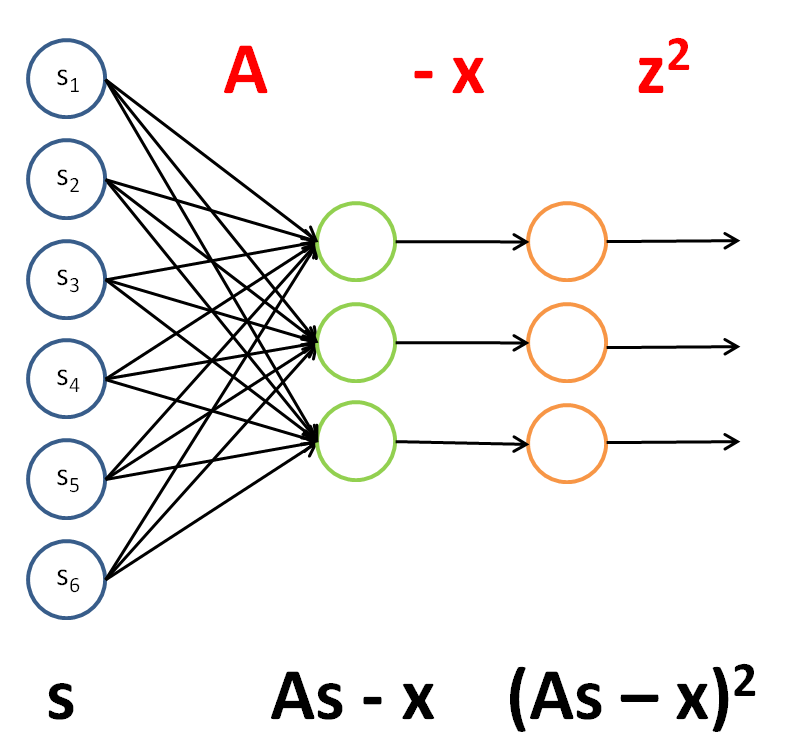
\includegraphics[width=0.4\textwidth]{figures/Backpropagation_Method_Example_1.png}
  %\caption{}\label{fig:step1}
\end{figure}

\cnt{The weights and activation functions of this network are as follows:}
    {该网络的权重和激励函数如下表所示:}
    {}

\begin{table}[h] \centering
%\caption{table1} \label{tab:table1}
\begin{tabular}{|c|c|c|}
  \hline
  \textbf{\cnt{Layer}{层}{}} & \textbf{\cnt{Weight}{权重}{}} & \textbf{\cnt{Activation function $f$}{激励函数$f$}{}} \\

  \hline
  1 & $A$ & $f(z_i) = z_i$ \cnt{(identity)}{(单位函数)}{} \\
  \hline
  2 & $I$ \cnt{(identity)}{(单位向量)}{} & $f(z_i) = z_i - x_i$ \\
  \hline
  3 & N/A & $f(z_i) = z_i^2$ \\

  \hline
\end{tabular} \\[10pt]
\end{table}

\cnt{To have $J(z(3)) = F(x)$, we can set $J(z^{(3)}) = \sum_k J(z^{(3)}_k)$.}
    {为了使 $J(z(3)) = F(x)$,我们可令 $J(z^{(3)}) = \sum_k J(z^{(3)}_k)$ 。}
    {}

\cnt{Once we see $F$ as a neural network, the gradient $\nabla_X F$ becomes easy to compute - applying backpropagation yields:}
    {一旦我们将 $F$ 看成神经网络,梯度 $\nabla_X F$ 就很容易求了——使用反向传导得到:}
    {}

\begin{table}[h] \centering
%\caption{table1} \label{tab:table1}
\begin{tabular}{|c|m{0.23\textwidth}|c|m{0.14\textwidth}|}
  \hline
  \textbf{\cnt{Layer}{层}{}} & \textbf{\cnt{Derivative of activation function $f'$}{激励函数的导数$f'$}{}} & \textbf{Delta} & \textbf{\cnt{Input $z$ to this layer}{该层输入$z$}{}} \\

  \hline
  3 & $f'(z_i) = 2z_i$ & $f'(z_i) = 2z_i$ & $As - x$ \\
  \hline
  2 & $f'(z_i) = 1$    & $\left( I^T \delta^{(3)} \right) \bullet 1$ & $As$ \\
  \hline
  1 & $f'(z_i) = 1$    & $\left( A^T \delta^{(2)} \right) \bullet 1$ & $s$ \\

  \hline
\end{tabular} \\[10pt]
\end{table}

\cnt{Hence,}
    {因此}
    {}
\begin{align} \nabla_X F & = A^T I^T 2(As - x) \\ & = A^T 2(As - x) \end{align} 



\textbf{\cnt{Example 2: Smoothed topographic L1 sparsity penalty in sparse coding}{示例2:稀疏编码中的平滑地形L1稀疏罚函数}{}}

\cnt{Recall the smoothed topographic L1 sparsity penalty on $s$ in sparse coding(\ref{chp:sparsecodingautoencinterp}):}
    {回顾 稀疏编码(\ref{chp:sparsecodingautoencinterp}) 一节中对 $s$ 的平滑地形L1稀疏罚函数:}
    {}
$$
\sum{ \sqrt{Vss^T + \epsilon}} 
$$
\cnt{where $V$ is the grouping matrix, $s$ is the feature matrix and $\epsilon$ is a constant.}
    {其中 $V$ 是分组矩阵, $s$ 是特征矩阵, $\epsilon$ 是一个常数。}
    {}

\cnt{We would like to find $\nabla_s \sum{ \sqrt{Vss^T + \epsilon}}$. As above, let's see this term as an instantiation of a neural network:}
    {我们希望求得 $\nabla_s \sum{ \sqrt{Vss^T + \epsilon}}$。像上面那样,我们把这一项看做一个神经网络的实例:}
    {}

\begin{figure}[ht] \centering
  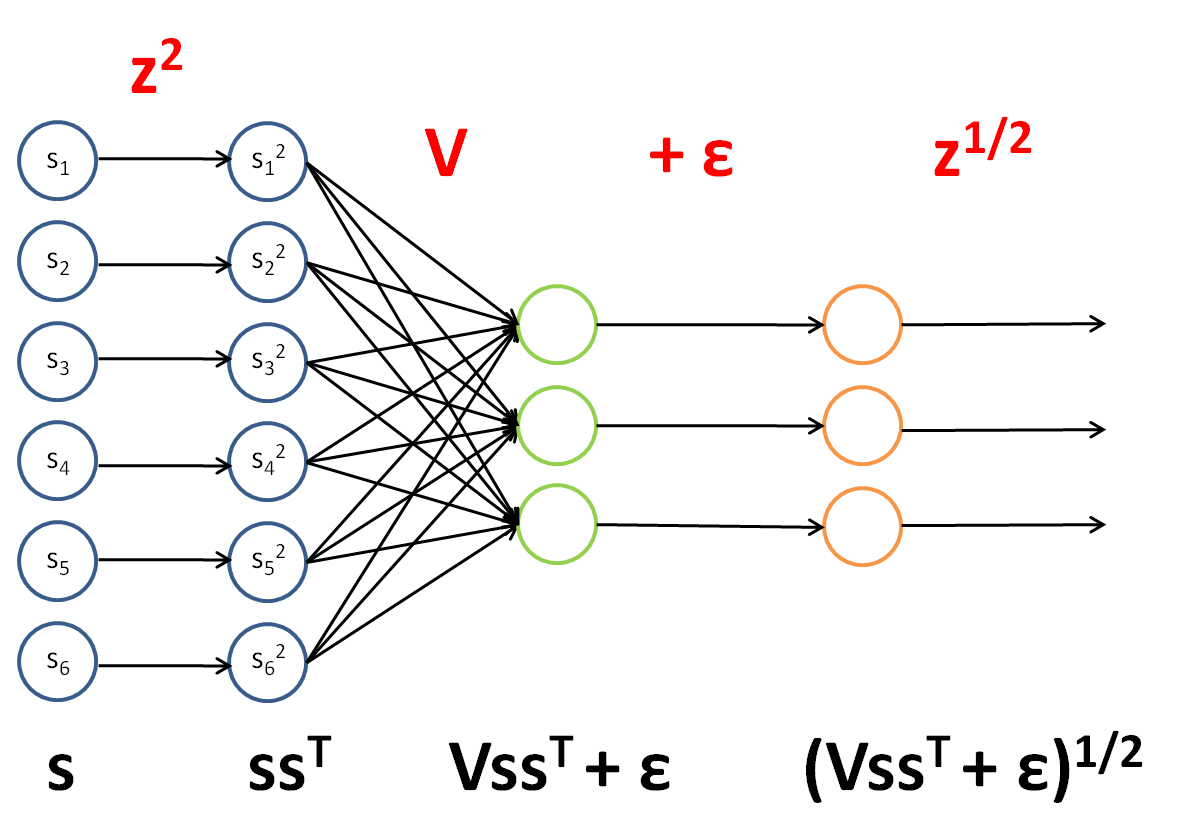
\includegraphics[width=0.5\textwidth]{figures/Backpropagation_Method_Example_2.png}
  %\caption{}\label{fig:step1}
\end{figure}

\cnt{The weights and activation functions of this network are as follows:}
    {该网络的权重和激励函数如下表所示:}
    {}

\begin{table}[h] \centering
%\caption{table1} \label{tab:table1}
\begin{tabular}{|c|c|c|}
  \hline
  \textbf{\cnt{Layer}{层}{}} & \textbf{\cnt{Weight}{权重}{}} & \textbf{\cnt{Activation function $f$}{激励函数$f$}{}} \\

  \hline
  1 & $I$ & $f(z_i) = z_i^2$ \\
  \hline
  2 & $V$ & $f(z_i) = z_i$ \\
  \hline
  3 & $I$ & $f(z_i) = z_i + \epsilon$ \\
  \hline
  4 & N/A & $f(z_i) = z_i^{\frac{1}{2}}$ \\

  \hline
\end{tabular} \\[10pt]
\end{table}

\cnt{To have $J(z(4)) = F(x)$, we can set $J(z^{(4)}) = \sum_k J(z^{(4)}_k)$.}
    {为使 $J(z(4)) = F(x)$,我们可令 $J(z^{(4)}) = \sum_k J(z^{(4)}_k)$。}
    {}

\cnt{Once we see $F$ as a neural network, the gradient $\nabla_X F$ becomes easy to compute - applying backpropagation yields:}
    {一旦我们把 $F$ 看做一个神经网络,梯度 $\nabla_X F$ 变得很容易计算——使用反向传导得到:}
    {}

\begin{table}[h] \centering
%\caption{table1} \label{tab:table1}
\begin{tabular}{|c|m{0.23\textwidth}|c|m{0.14\textwidth}|}
  \hline
  \textbf{\cnt{Layer}{层}{}} & \textbf{\cnt{Derivative of activation function $f'$}{激励函数的导数$f'$}{}} & \textbf{Delta} & \textbf{\cnt{Input $z$ to this layer}{该层输入$z$}{}} \\

  \hline
  4 & $f'(z_i) = \frac{1}{2} z_i^{-\frac{1}{2}}$ & $f'(z_i) = \frac{1}{2} z_i^{-\frac{1}{2}}$ & $(Vss^T + \epsilon)$ \\
  \hline
  3 & $f'(z_i) = 1$ & $\left( I^T \delta^{(4)} \right) \bullet 1$ & $Vss^T$ \\
  \hline
  2 & $f'(z_i) = 1$ & $\left( V^T \delta^{(3)} \right) \bullet 1$ & $ss^T$ \\
  \hline
  1 & $f'(z_i) = 2z_i$ & $\left( I^T \delta^{(2)} \right) \bullet 2s$  & $s$ \\

  \hline
\end{tabular} \\[10pt]
\end{table}

\cnt{Hence,}
    {因此}
    {}
\begin{align} \nabla_X F & = I^T V^T I^T \frac{1}{2}(Vss^T + \epsilon)^{-\frac{1}{2}} \bullet 2s \\ & = V^T \frac{1}{2}(Vss^T + \epsilon)^{-\frac{1}{2}} \bullet 2s \\ & = V^T (Vss^T + \epsilon)^{-\frac{1}{2}} \bullet s \end{align} 


\textbf{\cnt{Example 3: ICA reconstruction cost}{示例3:ICA重建代价}{}}

\cnt{Recall the independent component analysis (ICA \ref{chp:indepcomponanalysis}) reconstruction cost term: $\lVert W^TWx - x \rVert_2^2$ where $W$ is the weight matrix and $x$ is the input.}
    {回顾 独立成分分析(ICA \ref{chp:indepcomponanalysis}) 一节重建代价一项: $\lVert W^TWx - x \rVert_2^2$,其中 $W$ 是权重矩阵, $x$ 是输入。}
    {}

\cnt{We would like to find $\nabla_W \lVert W^TWx - x \rVert_2^2$ -- the derivative of the term with respect to the weight matrix, rather than the input as in the earlier two examples. We will still proceed similarly though, seeing this term as an instantiation of a neural network:}
    {我们希望计算 $\nabla_W \lVert W^TWx - x \rVert_2^2$ -- 对于权重矩阵的导数,而不是像前两例中对于输入的导数。不过我们仍然用类似的方法处理,把该项看做一个神经网络的实例:}
    {}

\begin{figure}[ht] \centering
  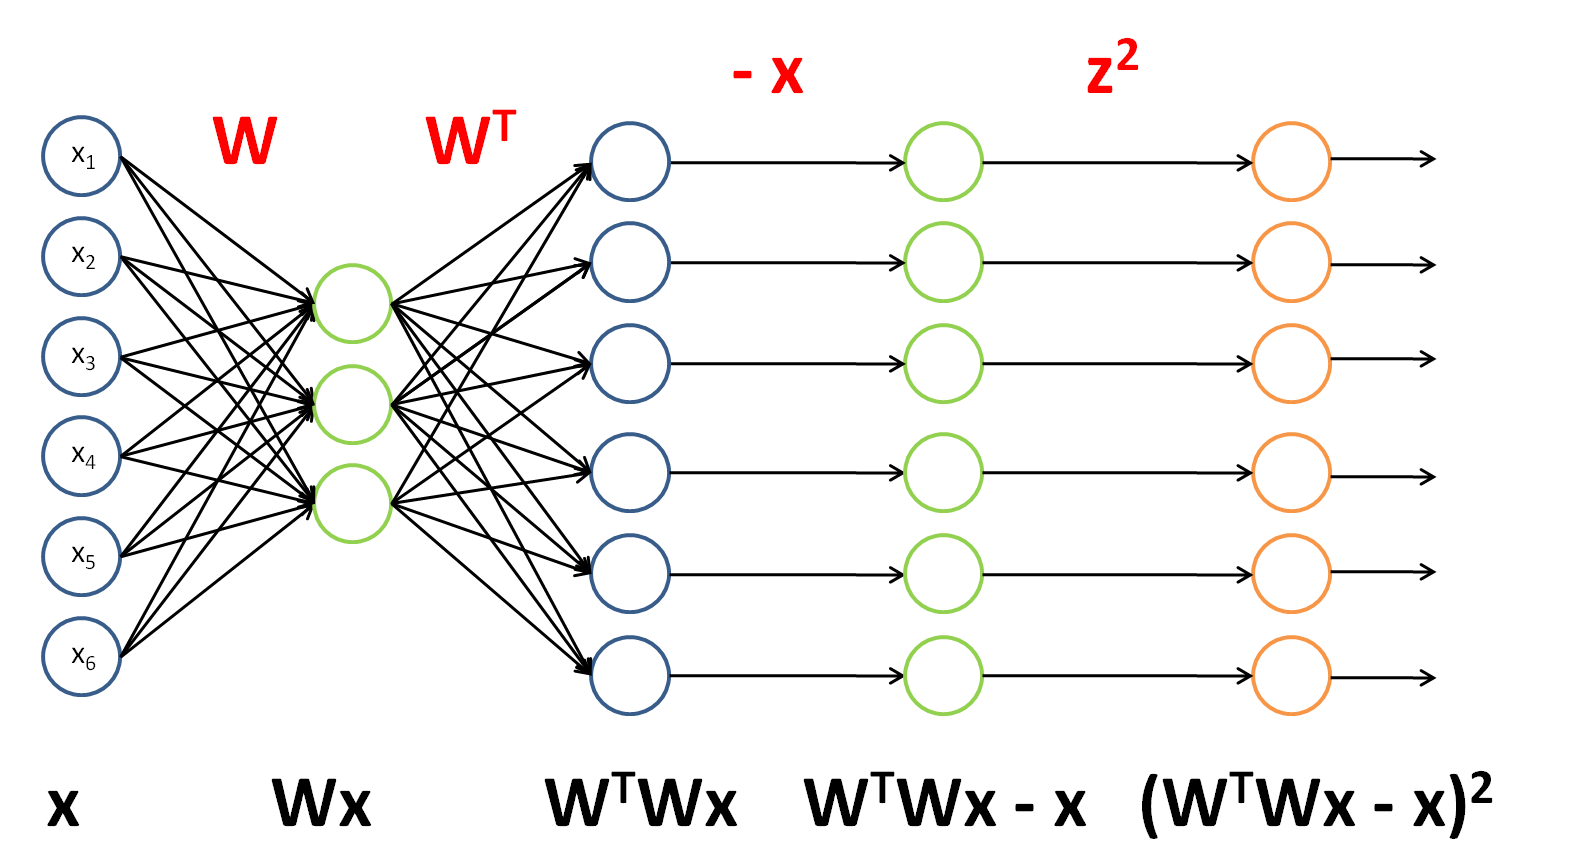
\includegraphics[width=0.6\textwidth]{figures/Backpropagation_Method_Example_3.png}
  %\caption{}\label{fig:step1}
\end{figure}

\cnt{The weights and activation functions of this network are as follows:}
    {该网络的权重和激励函数如下表所示:}
    {}

\begin{table}[h] \centering
%\caption{table1} \label{tab:table1}
\begin{tabular}{|c|c|c|}
  \hline
  \textbf{\cnt{Layer}{层}{}} & \textbf{\cnt{Weight}{权重}{}} & \textbf{\cnt{Activation function $f$}{激励函数$f$}{}} \\

  \hline
  1 & $W$   & $f(z_i) = z_i$ \\
  \hline
  2 & $W^T$ & $f(z_i) = z_i$ \\
  \hline
  3 & $I$   & $f(z_i) = z_i - x_i$ \\
  \hline
  4 & N/A   & $f(z_i) = z_i^2$ \\

  \hline
\end{tabular} \\[10pt]
\end{table}

\cnt{To have $J(z(4)) = F(x)$, we can set $J(z^{(4)}) = \sum_k J(z^{(4)}_k)$.}
    {为使 $J(z(4)) = F(x)$,我们可令 $J(z^{(4)}) = \sum_k J(z^{(4)}_k)$ 。}
    {}

\cnt{Now that we can see $F$ as a neural network, we can try to compute the gradient $\nabla_W F$. However, we now face the difficulty that $W$ appears twice in the network. Fortunately, it turns out that if $W$ appears multiple times in the network, the gradient with respect to $W$ is simply the sum of gradients for each instance of $W$ in the network (you may wish to work out a formal proof of this fact to convince yourself). With this in mind, we will proceed to work out the deltas first:}
    {既然我们可将 $F$ 看做神经网络,我们就能计算出梯度 $\nabla_W F$ 。然而,我们现在面临的难题是 $W$ 在网络中出现了两次。幸运的是,可以证明如果 $W$ 在网络中出现多次,那么对于 $W$ 的梯度是对网络中每个 $W$ 实例的梯度的简单相加(你需要自己给出对这一事实的严格证明来说服自己)。知道这一点后,我们将首先计算delta:}
    {}

\begin{table}[h] \centering
%\caption{table1} \label{tab:table1}
\begin{tabular}{|c|m{0.23\textwidth}|c|m{0.14\textwidth}|}
  \hline
  \textbf{\cnt{Layer}{层}{}} & \textbf{\cnt{Derivative of activation function $f'$}{激励函数的导数$f'$}{}} & \textbf{Delta} & \textbf{\cnt{Input $z$ to this layer}{该层输入$z$}{}} \\

  \hline
  4 & $f'(z_i) = 2z_i$ & $f'(z_i) = 2z_i$ & $(W^TWx - x)$ \\
  \hline
  3 & $f'(z_i) = 1$ & $\left( I^T \delta^{(4)} \right) \bullet 1$ & $W^TWx$ \\
  \hline
  2 & $f'(z_i) = 1$ & $\left( (W^T)^T \delta^{(3)} \right) \bullet 1$ & $Wx$ \\
  \hline
  1 & $f'(z_i) = 1$ & $\left( W^T \delta^{(2)} \right) \bullet 1$ & $x$ \\

  \hline
\end{tabular} \\[10pt]
\end{table}

\cnt{To find the gradients with respect to $W$, first we find the gradients with respect to each instance of $W$ in the network.}
    {为计算对于 $W$ 的梯度,首先计算对网络中每个 $W$ 实例的梯度。}
    {}

\cnt{With respect to $W^T$:}
    {对于 $W^T$:}
    {}
\begin{align} \nabla_{W^T} F & = \delta^{(3)} a^{(2)T} \\ & = 2(W^TWx - x) (Wx)^T \end{align} 

\cnt{With respect to $W$:}
    {对于 $W$:}
    {}
\begin{align} \nabla_{W} F & = \delta^{(2)} a^{(1)T} \\ & = (W^T)(2(W^TWx -x)) x^T \end{align} 

\cnt{Taking sums, noting that we need to transpose the gradient with respect to $W^T$ to get the gradient with respect to $W$, yields the final gradient with respect to $W$ (pardon the slight abuse of notation here):}
    {最后进行求和,得到对于 $W$ 的最终梯度,注意我们需要对 $W^T$ 梯度进行转置,来得到关于 $W$ 的梯度(原谅我在这里稍稍滥用了符号):}
    {}

\begin{align} \nabla_{W} F & = \nabla_{W} F + (\nabla_{W^T} F)^T \\ & = (W^T)(2(W^TWx -x)) x^T + 2(Wx)(W^TWx - x)^T \end{align} 


\section{\cnt{Miscellaneous}{}{}}

\subsection{\cnt{MATLAB Modules}{}{}}

Sparse autoencoder | \href{http://ufldl.stanford.edu/wiki/resources/sparseae_exercise.zip}{sparseae\_exercise.zip}
\begin{itemize}
  \item checkNumericalGradient.m - Makes sure that computeNumericalGradient is implmented correctly
  \item computeNumericalGradient.m - Computes numerical gradient of a function (to be filled in)
  \item display\_network.m - Visualizes images or filters for autoencoders as a grid
  \item initializeParameters.m - Initializes parameters for sparse autoencoder randomly
  \item sampleIMAGES.m - Samples $8 \times 8$ patches from an image matrix (to be filled in)
  \item sparseAutoencoderCost.m - Calculates cost and gradient of cost function of sparse autoencoder
  \item train.m - Framework for training and testing sparse autoencoder 

\end{itemize}

Using the MNIST Dataset | \href{http://ufldl.stanford.edu/wiki/resources/mnistHelper.zip}{mnistHelper.zip}

\begin{itemize}
  \item loadMNISTImages.m - Returns a matrix containing raw MNIST images
  \item loadMNISTLabels.m - Returns a matrix containing MNIST labels 
\end{itemize}

PCA and Whitening | \href{http://ufldl.stanford.edu/wiki/resources/pca_exercise.zip}{pca\_exercise.zip}

\begin{itemize}
  \item display\_network.m - Visualizes images or filters for autoencoders as a grid
  \item pca\_gen.m - Framework for whitening exercise
  \item sampleIMAGESRAW.m - Returns $8 \times 8$ raw unwhitened patches 
\end{itemize}

Softmax Regression | \href{http://ufldl.stanford.edu/wiki/resources/softmax_exercise.zip}{softmax\_exercise.zip}

\begin{itemize}
  \item checkNumericalGradient.m - Makes sure that computeNumericalGradient is implmented correctly
  \item display\_network.m - Visualizes images or filters for autoencoders as a grid
  \item loadMNISTImages.m - Returns a matrix containing raw MNIST images
  \item loadMNISTLabels.m - Returns a matrix containing MNIST labels
  \item softmaxCost.m - Computes cost and gradient of cost function of softmax
  \item softmaxTrain.m - Trains a softmax model with the given parameters
  \item train.m - Framework for this exercise 
\end{itemize}


\subsection{\cnt{Style Guide}{}{}}


\textbf{File / Function Names}

Functions and file names should be alphanumeric, with the first letter of the first word in lowercase, and the first letter in the remaining words in uppercase. E.g.


\textbf{Variable Names}

Variable names should follow the same convention as the style guide. 



\subsection{\cnt{Useful Links}{}{}} \label{chp:usefullinks}


\href{http://www.stat.berkeley.edu/~spector/matlab.pdf}{Matlab Guide}

\href{http://www.mathworks.com/matlabcentral/fx_files/5685/2/matopt.zip}{Writing Fast MATLAB Code (by Pascal Getreuer)}

\href{http://www.psi.toronto.edu/matrix/calculus.html}{Matrix Calculus Reference}

\href{http://www.imm.dtu.dk/pubdb/views/edoc_download.php/3274/pdf/imm3274.pdf}{The Matrix Cookbook}

\href{http://www.math.duke.edu/~jvb/papers/cnn_tutorial.pdf}{Notes on Convolutional Neural Networks}
